\articlepart{我流運指 underground}{o-ck}

\section{はじめに}

“我流運指”という言葉、聞いたことがおありでしょうか?
タイピング愛好者、いわゆるタイパーならば、どこかで耳にしたことがあるかもしれませんが、
そうでない方々とってはあまり馴染みのない言葉かもしれません。
簡単に言ってしまえば、“ちょっと変わった指使いでのタイピング”といったところです。

タイピングという言葉をわざわざ持ってこなくても、パソコンを普段使っている方々であれば、
「キーボードを打鍵する」という行為は、生活の一部と言って良いほど日常的に行っている行為だと思います。

当然、人によってそのときの指使い、すなわち運指というものは千差万別でしょう。
同じ単語を打つにしても、5人に尋ねて5人が全員違う運指だった、ということもありました。

一方で、キーボードの打ち方には“標準運指”と呼ばれているものがあります。
\key{F}キーと\key{J}キーに人差し指を置き、それを基点として、外側に向かって順々に
中指、薬指、小指を置いて、両親指以外の8本で満遍なくキーを打鍵するというものです(親指はスペースキーを打つ)。
市販のタイピングソフトのようなものは、
恐らくこの標準運指に従って練習が組み立てられているでしょう。

一見すると、標準運指は満遍なく8本の指を全体的に均等に使うため、
高速でタイピングを行うには、何も欠点がないように思われます。
…しかし、世の中にはそうでない、ちょっと変わった運指を駆使して
高速タイピングに挑み続ける者たちもいるのです
(この記事では、そのような方々のことを“我流タイパー”と呼ぶこととします)。

この記事では、標準運指と比較すると少し異端なものとして捉えられがちな
“我流運指”にあえて焦点を当て、我流運指についての考察、
ならびにそのタイピングの可能性について述べていきたいと思います。

こういった、ちゃんとした文章を書くことには慣れていないので、
一部お見苦しい箇所もあるかもしれませんが…。まぁ、アラカルト的な内容ということで、
肩の力を抜いて気楽に読んで頂ければと思います~。\\

☆本文に入る前に…\\

\subsection*{この記事は、「我流運指を薦めるもの」、「上達を目指すアドバイス」ではありません}

タイピング本に掲載されている記事ということならば、読めば上達に繋がるのではと
多くの読者は思われるかもしれません。…が、残念ながらこの記事に限っては、
読むことで上達に繋げられる可能性は薄いかと思われます(笑)

それでは、この記事では読者に何を訴えたいかというと、まず標準運指の方や
それに近い運指の方には、単に「こんな変な運指でも、よく考えてみれば
理に適った打ち方をしているし、真面目に打ち込んでる人は居るんだ!」
ということ。


そして、我流運指の方には、本記事での運指の考察を通すことで
自分自身の運指についての理解、または共感を一つでも多く感じていただければ、と思います。
もしかしたら、新たな運指を編み出すきっかけになるかも…!?

\subsection*{この記事は、Qwerty配列についてのみ取り扱います}

理由は簡単で、私自身Qwerty配列しか使ったことがないからです(笑)
JISかな打ちも経験したことがないため、議論の対象はQwerty配列での
日本語ローマ字打ち、ないし英文打ちについて、ということになります。


\section{我流運指とはなにか?}

\subsection{“我流”の意味}

本記事全体に関わってくる言葉ということで、まずは最初に“我流運指”という言葉の定義について
以下のように述べておこうと思います。\\

『我流運指とは、標準運指と異なる運指である。』\\

\noindent …と、いきなり言われても「えっ、こんな曖昧な定義でいいの!?」と感じられるかもしれません。
しかし、このような曖昧な定義にならざるを得ないのには理由があります。

一般的には、我流運指という言葉は“標準運指”の対義語的に使われていることが多いと感じます。
しかし、標準運指と言われているものは、ただひとつの決められた運指であり、
すべてのキーにわたって厳密に標準運指に従っている人は、そう多くないと予想されます。

それでは、どこからがいわゆる“我流”と呼べるのかと考えると、
“標準運指と大きく異なる運指”というような、曖昧な定義しかできないという発想に至ったからです。
例えば、以下のようなケースが考えられます。
\begin{itemize}
 \item 普段は標準運指だが、ある特定の文字列を打つときのみ、標準運指とは異なる運指に変わる。
 \item キーによって、標準運指に準拠しているところと、そうでないところがある。
\end{itemize}
このような2つのケースにおいて、「我流運指と呼ぶべきか、否か」という問いに対して
厳密な答えを与えること、つまり“我流運指の厳密な定義付け”を行うのは非常に難しいですし、
そこにはあまり意味がないと思います。

やや乱暴な例ですが、「標準運指と○ヶ所異なる運指を我流運指と呼ぶ」と定義したとしても、
どこから我流運指として捉えるかは、完全に個人の感覚次第です。
そのため、先述のような曖昧さを残した定義しかできないと考えました。
かといって、「個人の感覚次第」とだけ結論づけてしまうのも少し寂しいですし、
本記事を書くにあたって、何らかの定義がないと不便であると感じたので、
この章の冒頭のような定義を考えました。

しかし、冒頭の定義はかなり曖昧なものであるため、一般的に捉えられている
“我流”のイメージとは少し離れてしまっているかもしれません。
そこで、次のように定義を拡張してみます。\\

『我流運指とは、
狭義には「標準運指と大きく異なる運指」であり、
広義には「標準運指と異なる運指」である。』\\

私が記事を書くことになって色々考えた結果気付いたのは、
「我流運指とは、小さな最適化、つまり“標準運指と異なる運指”が
積み重なった結果として表れるものではないか」ということです。
一見珍妙に見える運指でも、一つずつほどいていけば、「標準運指の状態から
最適化をいくつも重ねたもの」として捉えることができるのではないでしょうか。

たとえ1ヶ所だけの最適化でも、それは本人が「この運指のほうが打ちやすい」と思って
会得したものであるのだから、そういう意味では“我流”と呼んで良いと思います。
第3章では、実際に私が行っている最適化について考察していきますが、
標準運指に近い方でも、もしかしたら共感を得られるような最適化が
いくつかあるかもしれません。

そして、ここまで書いて気付いたけど…この記事ってもしかして、
我流運指じゃなくて最適化についての記事なのでは…!?
まぁ、細かいことは気にしないようにしましょう(笑)



\subsection{なぜ我流運指が生まれるのか}


タイピングにはマニュアルというものがありません。
操作を覚えるのではなく、自分の技能として身につけるものです。
…某タイピングサイトの例文より(笑)
でもこれはまったくその通りで、基本的には何回も反復練習することで
自分のものとして徐々に身に付けていくスキルだと思います。
標準運指の方には、運指が画面に表示されるようなタイピングソフトなどで
その通りに練習していくことで、身につけたという方も多いでしょう。

私の知る限りでは、いわゆる我流タイパーには、標準運指というものを知らないで
自由に打っているうちに身についた、という方が多いように思えます。
少数ですが、その逆のパターン、つまり標準運指から我流運指に転向したという
例もありましたが、これは“転向”というよりも、最適化を重ねるうちに
そのように変わっていったのではないかと考えます。


ここで、我流運指が生まれる理由について考えてみましょう。
私が考えたのは、それらは大きく分けて、無意識的、意識的なものに
大別されるというものです。
例として挙げるとすれば、以下のようなものが考えられます。\\

[無意識的]
\begin{itemize}
 \item パソコンを初めて使い始めてから、何も意識せずに使っているうちにタイピングを覚えた
 \item 何回も同じ単語を打っているうちに、自然と打ちやすい運指に変わっていった
\end{itemize}

[意識的]
\begin{itemize}
 \item 打ちづらい単語に苦痛を覚え、研究してより打ちやすい運指を編み出した
 \item 他人の運指を見て、この方がより効率的だと思い、自分も導入した\\
\end{itemize}

他にも色々考えられるかもしれませんが、いずれの理由にしても共通して根幹にあるのは一つで、
それは“より自分に合った打ち方を考えている”という発想から来ているというものです。
ところが、ここで「自分に合った打ち方」というのは、必ずしも「速く打つことができる」ということに
直結はしないという点に注意が必要です。
というのは、我流運指においては自分が良かれと思って導入した最適化でも、
タイムを競うとなると、全体の結果としてはデメリットに働いてしまう例も
考えられるからです。

\section{私の考える運指論}

それでは、この章からは実際に例となる単語を挙げたりしながら、
具体的に私がどのような最適化を行っているかを前半で紹介しつつ、
後半ではそれをもとに私が考えている運指論を述べていきたいと思います。

\subsection{“人中”理論とは}

恐らく、誰も聞いたことがない言葉だと思います。でもそれは当然で、
私がこの記事を書くことになり、初めて作った言葉だからです(笑)
『じんちゅう』ではなく『ひとなか』とお読み下さい。
きっと多くの方がなんとなくお分かりになるかと思いますが、
これは人差し指と中指のことを指しています。
私の運指において特徴的だと思うのは、
\begin{itemize}
 \item 極端に人差し指、中指の占めるウェイトが大きい
 \item 1つのキーに対して、複数の指が担当することが多い
 \item その中でも人差し指、中指が担当するキーが非常に多い
\end{itemize}
ということだと思います。1つのキーに対して、前後の流れによって
人差し指、中指、薬指の3本の指が入れ代わり立ち代わりで
担当することが、日常のタイピングでもしばしばあります。
\subsubsection*{例:日本語}
\begin{itemize}
 \item 手帳 / tetyou / \finger{433487}
 \item 我々 / wareware / \finger{43434343}
 \item わざわざ / wazawaza / \finger{43434343}
 \item ぽわぽわ / powapowa / \finger{87438743}
 \item ふさわしい / husawasii / \finger{784343488}
 \item オピニオン / opinionn / \finger{78778877}
 \item イーサネット / i-sanetto / \finger{784373448}
\end{itemize}
\subsubsection*{例:英語}
\begin{itemize}
 \item award / \finger{34343}
 \item option / \finger{784787}
 \item excess / \finger{344333}
 \item museum / \finger{783487}
 \item stewardess / \finger{3434343433}
\end{itemize}

さてさて、私が実際に打っている運指の中で
特に特徴的と思われる運指をピックアップしてみましたが…。
\finger{3}、\finger{4}、\finger{7}、\finger{8}が多すぎて目がチカチカするかもしれませんね。
これは、つまり両人差し指および中指を多用していることを表しているのですが…
はい、あえてそういうワードを意図的に選んでみました(笑)


こうして書き出してみると、やはり外側のキー、つまり標準運指において
薬・小指が担当するキーを、無理やりにでも人・中指で押そうとする、
もはや執念と言って良いほどの強い意思が働いてるように思えますね。
図\ref{fig1_unsiock}に、私の運指表を掲載しました。(図\ref{fig1_unsiock})

\begin{figure*}
 \begin{center}
   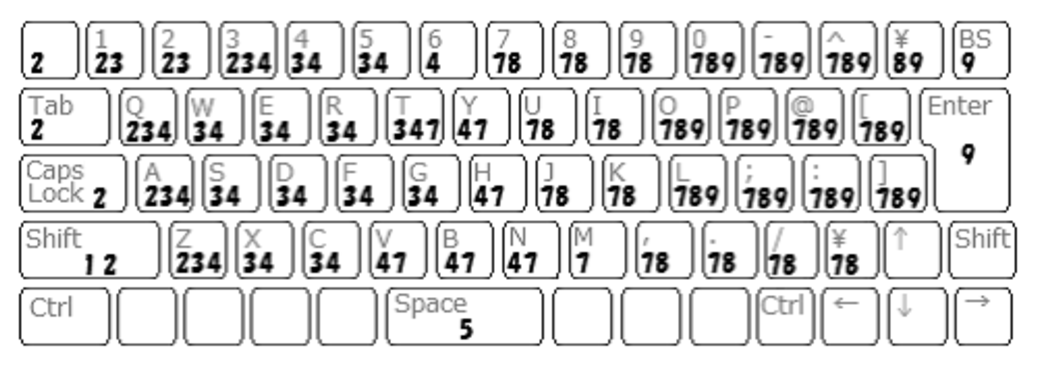
\includegraphics[width=14cm,clip]{res_o_ck/fig1_unsiock.eps}
 \end{center}
 \caption{運指表(o-ck)}
 \label{fig1_unsiock}
\end{figure*}

図に示されているように、標準運指など知ったこっちゃないフリーダム運指です(笑)
一つのキーに2本以上の指(主に人差し指、中指)が担当するのは当たり前で、右側の記号系のキーは
それに薬指が混じることもありますが、正直気分次第で適当に打っています。タイプウェルオリジナルの「すべてのキー」を
打っている時の運指は、自分でもほとんど把握できていません(人差し指、中指が多いとは思いますが…)。


なぜこのような運指になってしまったのかを自分なりに解釈してみると、
まず私のタイピングのコンセプトとして、“人差し指と中指こそが最も動かしやすい指である”というのが強く根底にあったからです。
これはタイプウェルを本格的に打ち込み始めてからではなく、
それこそパソコンに初めて触れ始め、キーボードを打つようになってから
自然に芽生えた考え方だと、今になって思います。
もちろん、当時は標準運指という存在なんて知りませんでしたから、
日々のネット生活の中で、人差し指と中指を中心にした運指が
自然と構築されていったというわけです。


実際、人差し指と中指は動かしやすい指であるために、タイピングには何も不便は感じませんでしたし、
それよりも「なぜわざわざ動かしにくい薬指や小指を使うのか?」という思いから、
薬指や小指を積極的に使おうという発想はありませんでした。
当然“\key{F}キーと\key{J}キーがホームポジションである”ということもまったく知りませんでしたから、
「wa」と打ちたければ\finger{4}→\finger{3}が飛んでいきますし、「o-」と打ちたければ、
これまた\finger{7}→\finger{8}が飛んでいくのです。ホームポジションを知らないが故の、
いわば“自由度”がこのような運指を育んだのだろうと思います。


このように、動かしづらい薬指、小指を徹底的に排除し、動かしやすい人差し指および
中指を駆使して無理やりにでも最適化してやろうというのが、私のタイピングスタイルです。
このような理論を、“人中”(ひとなか)理論と名付けてみました。


\subsection{すべてが“人中”ではない}

先ほど、日本語と英語でそれぞれいくつか運指の例を挙げましたが、
あれほど4つの数字が並んだ運指だけを挙げると、すべてのキーを
人差し指か中指で打っているのかと思われるかもしれませんが、
実際はそんなことはありません。
確かに、人差し指と中指はウェイトを多く占めてはいますが、
前後の文字列など、いくつかの例外ルールに従って薬指を使うこともあります。

このセクションでは、“人中”理論に付随するものとして、
その他の親指、薬指、小指について説明を加えたいと思います。

\subsubsection*{左薬指について}

単語の入力において、左手および右手を含め、薬指を使う頻度が最も高いのは
ずばり、\key{A}キーです。これはキーボードの端にあるということだけでなく、
日常でもかなり使用頻度が高いキーであるという2つの理由が重なっているためです。

「wa」「za」「sa」はすべて\finger{4}→\finger{3}ですが、“人中”理論によるこの例は
\key{A}キー直前の子音が隣接するキーであるからであって、
むしろ\key{A}キーが中指を担当するのは例外的とも言えます。
「ra」「ta」「fa」のように、直前の子音が少し離れた位置にあると
\finger{4}→\finger{3}では手の構造的に少し辛くなるので、\finger{4}→\finger{2}となります。

さらに、「ka」のように子音が右手担当の場合も、普段\key{A}キーの近くには
薬指があるので、薬指が担当することがほとんどです。
しかし「川(kawa)」「傘(kasa)」のような単語のときは、“人中”理論に
移行することとなります(運指はいずれも\finger{7343})。


左薬指を使用するもう一つの例としては、繋がりをスムーズにするためのものが
あります。使用する単語の例は、「視聴(sityou)」など。
この場合は、「si」の後に続く「ty」を\finger{3}→\finger{4}で打ちたいという意識が働くため、
\key{S}キーを人差し指や中指で打つよりも、薬指で打ったほうが
「ty」以降のまとまりに移行する時間を短縮できるからです。

しかし、これと似たような「怒張(dotyou)」という単語を考えた時、
\key{D}キーは中指が出てきます。\key{D}→\key{T}は同じ中指が担当するわけですが、
これにかかる移動時間は自分の中で許容範囲、つまり苦にならないレベルと
判断されるためです。


\subsubsection*{右薬指について}

左手に比べると頻度はまた下がりますが、右手の薬指も、単語によっては
重要になってきます。例えば、「o-」は単独で来た場合は\finger{7}→\finger{8}ですが、
「jo-」「no-」「mo-」のように\key{O}キーの左下付近にある子音と
組み合わさった場合は、\finger{7}→\finger{8}→\finger{9}となることが多いです。
(稀に気分次第で、左人差し指が\key{N}\key{M}キーまで出張してくることも…(笑))
しかし、この場合は人差し指や中指、または\key{A}キーにおける薬指よりも
使用頻度がだいぶ少ないため、正確性は下がってしまいます。

右薬指の場合も、先ほどの左薬指の場合と同様に、繋がりをスムーズに
するためのものがあります。単語の例としては「over」など。
「over」の運指を書き下すと、\finger{9734}となります。この場合も
「ov」の後に続く「er」を\finger{3}→\finger{4}で打ちたいという強い意思のもと、
「ov」をひとかたまりで打ちたいと思うのですが、人差し指と中指では
手の形が辛くなるので、薬指が出てくるというわけです。


「素直に『ver』を\finger{434}で打てば…」と、私自身記事を書きながら思いましたが、
長年染み付いた癖というものは恐ろしいもので…(笑)


\subsubsection*{その他の指(親指・小指)について}

正直、自分のタイピングにおいては完全に空気となっています。
…と最近まで思っていましたが、よくよく考えると、これらの指も
無くてはならない存在であることにふと気が付きました(笑)

まずは親指ですが、左親指は\key{Space}キー担当として立派に役目を果たしています。
タイプウェルを熱心にやり込んでいた2006年頃までは、実は\key{Space}キーは
人差し指が担当していました(日常でもそうであったかは、今となっては覚えていません)。

しかし、しばらくタイピングから離れているうちに、とっても久しぶりに
タイプウェルを起動してみたところ、いつの間にか親指スペースが染み付いており、
「以前のタイピングができなくなった…」と、これもモチベ消失の原因の一つでした(笑)

今となっては、なぜ人差し指スペースであの記録を出せたのか訳が分からないというくらいに
親指スペースは便利だと感じていますし、事実、1ワードあたりの打鍵数が少ない
英単語において、当時より大幅に記録を伸ばすことができたので、
やはり親指スペースが使えるに越したことはないと痛感しています。


次に、小指についてですが、これは\key{Shift}キー担当として重要でした。
ちなみに私はいかなる状況でも左の\key{Shift}キーしか使っていませんが、
これはパソコンを覚えたての自分が、そもそも右にも\key{Shift}キーがあることを
知らなかったためでしょう(笑)

しかしそんな左\key{Shift}キーも、たまに薬指担当になることもあります。
「American」なんかがパッと思いついた例ですが、この場合は「A」という文字を
「大文字のA」としてではなく、「Shift→ A」という一連の流れとして
見ているため、使いにくい小指よりも薬指が気分次第で出てくるものと思います。


ちなみに句読点\key{,}\key{.}は人差し指、その他カギカッコや
アットマーク、アンダーバーなどの記号系は、主に指の使いやすさから、
指の移動距離が遠くなろうとも、人差し指か中指で打つことがほとんどです。
…右手の親指と小指の出番は、一切無かった(キッパリ)


\subsection{“塊”の認識}

もう一つ、私のタイピングにおいて、運指決定に重要な因子があります。
それは、文字列をただの連続したアルファベット(もしくは日本語)として
認識するのではなく、スムーズな打鍵が達成できるように、脳内で無意識的に
要所要所で“切断”して、“塊”を作ってタイピングを行っているというものです。
言葉では説明しづらいと思いますが、百聞は一見にしかず、ということで
例を挙げれば納得していただけるかと思います。

「こてこて(kotekote)」「たじたじ(tajitaji)」は典型的な加速ワードとして
扱われることが多いですが、例えば「kotekote」を速く打とうと意識すると、
自然と[ko][te]という、片手で打てる2打鍵を“塊”として認識して、
右手、左手、右手、左手、というようにリズミカルに打とうという意識が働きませんか?

つまり、この場合では本来「kotekote」は8打鍵ですが、
2打鍵ずつをひと塊として認識することで、感覚としては
4アクションで1単語を打ち切っていると見なせます。
これが“塊”の一番分かりやすい例でしょう。

上に挙げた例では[子音+母音]ですが、これだけではなく
[母音+母音][子音+子音]の例も有り得ます。
また、人によっては、3打鍵をひと塊の感覚で打っているという方も
いらっしゃるかもしれません。


ここで、これらの説明を一度に行うのに最適な単語の例を
偶然にも発見してしまったので、早速取り上げたいと思います(笑)
それはこの章の最初、「3.1 “人中”理論とは」で取り上げた「手帳」の運指なのですが、
あらためて再掲します。
\begin{itemize}
 \item 手帳 / tetyou / \finger{433487}
\end{itemize}
この運指を見て、「なぜ1回目と2回目の\key{T}キーが違う指を担当しているのか?」
と疑問に思った方がいらっしゃったかもしれません。このような少し面倒臭い
運指になっているのは、“塊”の認識が働いているためです。
「tetyou」を塊ごとに分けてみると、[te][ty][ou]となります。
なんと都合が良いことに、「子音+母音」「子音+子音」「母音+母音」の
すべての組み合わせが揃っています!(笑)

これらの3ブロックはいずれも、単独で出てくることを考えた時に
人差し指、中指を使って一気に打ってしまったほうが速い文字列です。
そのため、まずは[te]を\finger{4}→\finger{3}で打ったら、次は[ty]を\finger{3}→\finger{4}で打つべく
少し左手を移動して、それを打ち切ったら間髪入れずに右手で[ou]を\finger{8}→\finger{7}で打つ…
というのが、「tetyou」を打つ時の一連の思考の流れです。


このような“塊”の認識は、一方で、自らの運指の自由度を縛ってしまう
こともあります。例えば、「めっぽう(meppou)」「一方(ippou)」などに
表れる「ppou」の文字列。
これは私の運指では\finger{8887}という運指になり、標準運指の\finger{0097}と比べると
やや非効率で、時間短縮という面でも効果がないように思えます。
実際、その通りだと思います。
しかし、理屈では分かっていても、[ou]という文字列は、その他の場合で
圧倒的に\finger{8}→\finger{7}の“塊”として認識することが多いため、中指が連続していても
\finger{8887}で打ったほうが、頭の中ではスムーズに処理されるのです。


これと同様な例としては「のっぽ(noppo)」など。運指を書き下すと
\finger{78887}となり、これまた中指が連続していて、詰まりやすいのではと
思われるかもしれません。
ところが、この場合でも[no][po]が人差し指、中指で一気に打てるものとして
普段から認識されているために、むしろ上記以外の運指でないと
かえって気持ち悪く感じてしまいます。



\subsection{その他の最適化}

この記事では、主に“運指の変更”による種々の最適化を取り扱っています。
最適化は、打鍵をスムーズに打つために行うものですが、運指の変更以外でも
場合によっては単語を打ちやすくする方法もあります。
それは、「く」を打つのに「ku」「cu」、「じ」を打つのに「ji」「zi」の
いずれでも良いという、Qwerty配列の仕様を用いるものです。

個人的にですが、最適化という言葉は、運指の変更を指す場合が多いように
感じており、「ku」「cu」の打ち分けなどのことを最適化と言うことが
正しいのかは定かではありませんが、いずれにせよ“打鍵をスムーズにする”
という目的は同じでしょう。
そのような観点から、ここではそのような打ち分けも最適化の一つと見なし、
補足的に説明しようと思います。
まず、最適化としてよく使われる打ち分けには、以下のようなものが挙げられます。\footnote{使用するIMEや、タイピングゲームによっては認識されないものもあります。}
\begin{itemize}
 \item 「か」:「ka」「ca」
 \item 「く」:「ku」「cu」
 \item 「こ」:「ko」「co」
 \item 「じ」:「ji」「zi」
 \item 「しゃ」:「sya」「sha」\footnote{「しゅ」「しょ」も同様。}
 \item 「ちゃ」:「tya」「cha」「cya」\footnote{「ちゅ」「ちょ」も同様。}
 \item 「ぁ」:「la」「xa」\footnote{「ぃ」~「ぉ」も同様。}
 \item 「せ」:「se」「ce」
\end{itemize}

なんとなく、私の使用頻度が高いものから順に並べてみました。
「か・く・こ」は他のものに比べて圧倒的に使用頻度が高いですが、
これは、それだけ日常で頻出する文字であるというだけでなく、
\key{K}よりも\key{C}を使ったほうが有利な場合が多いからです。

その反面、「cha」「ce」となると、ほとんど使った試しがありません。
「ちゃ」は「tya」のままで特に不便に感じていないためで、
「ce」はそもそもタイプウェルでは対応していないため、私には
馴染みがなかったからです。

なお、「し」を「si」ではなく「shi」と打つことでわざと打鍵数を水増しし、
e-typingなどのタイピングゲームで得点アップを狙うという攻略法も
あるのですが、これについては本記事の内容から外れるため、割愛させて頂きます。


「か・く・こ」を例に挙げると、この打ち分けによる利便性は、
\key{K}キーと\key{C}キーが大きく離れた場所、つまりキーボードの左側と右側に
位置していることに起因しています。
打ち分けを習得すれば、前後の文字列によって、どちらで打てばスムーズになるのか
\key{K}\key{C}の選択の幅が広がり、ワードによって減速を防いだり、
むしろ加速ワードにすることができるということも有り得ます。


具体的なワードを挙げると、「広告(koukoku)」。これは3回出現する\key{K}キーの
すべてが\key{C}キーで代用できます。つまり単純に考えて2×2×2、つまり8種類の打ち分けが可能です。
私自身は、「coucocu」とすべて\key{C}キーで打つことで、左右の手で分離して
リズミカルに打つことができるので、このような打ち方を採用しています。

人によって、例えば「oku」を塊として認識し、最適化しているような人であれば
「coucoku」のように最後の「oku」だけ\key{K}キーで打ち、\finger{9}→\finger{8}→\finger{7}の
最適化を行なっている、という最適化も考えられます。


「ji」「zi」もまた同様に、キーが左右にあるために、これも前後の流れによって
お好みで打ち分けをすることができます。

私の運指の場合では、「まじまじ(mazimazi)」の運指は\finger{73487348}、もしくは
\finger{72387238}となり、「こてこて」などが属するような超加速ワードに分類されます。
これは「majimaji」と打つよりも、\key{Z}キーを採用することによって
[az][im]の各ブロックを隣接した指で打つことができるようになり、
左右の手で分離することができるためです。

\key{J}キーで打ってしまうと、\key{M}→\key{J}キーで右人差し指の移動があるため、
トップスピードはやや劣ってしまいます。「『ji』を\finger{8}→\finger{9}で打てば?」と思われる
かもしれませんが、なるべく薬指は使いたくないということに加えて、
これだと左右の手が担当するブロックが[a][jim]のように分かれ、
アンバランスになってしまうため、非常に打ちづらくなると感じます。


最後に、「しゃ」についてですが、人によっては「sha」のほうが打ちやすく
感じられるかもしれません。これは、\key{Y}\key{H}キーはともに右人差し指の担当ですが、
単純に\key{H}キーのほうが中段に位置しているということで、移動距離が少ないためだと
考えられます。移動距離が少なければ、それだけミスの可能性も抑えられるでしょう。

また、これは後付けのような利点ですが、「sh」という文字列は英語において
頻出であるため、これに慣れておけば、将来的に英語を打つときも
スムーズに打てるようになる…かも?(笑)


\subsection{一般性への拡張へ向けて}

私が思うに、どんな珍妙な最適化、我流運指であっても、そこには何らかの
理由があるはずで、それは「2.2 なぜ我流運指が生まれるのか」で述べたような意識的、無意識的にかかわらず、
ある心理に従って形成されていくものではないでしょうか。
一口に“我流運指”と言っても、運指は人によって千差万別であるということは
この記事を書き始める段階で既に承知の上です。

しかし、我流運指について考えを詰めていくうち、我流運指というものは
すなわち最適化の積み重ねであり、色々な人の色々な最適化を広く見渡してみれば、
ある法則性や一般性のようなものが導けるのではないか、と考えました。


そこで、『一般性への拡張』について考察すべく、我流タイパーたち数人と
特殊運指について議論を交わしたりして、あれこれと考えていたのですが…。
もちろん有益な情報もたくさんあったのですが、多種多様な最適化の数々を
見ているうちに、「果たしてこれらは、“一般性”という簡単な言葉で
くくれるものだろうか?」と、疑心暗鬼に陥ってしまったのです(笑)
そのような理由から、記事として形にするに際しては、どうしても普遍性の高いものを
選ばざるを得なくなりましたが、私なりに考えたのは以下の三点です。


\subsubsection*{基本的には“クセ”}

我流タイパーには、「標準運指そっちのけで、自由に打ってるうちに
勝手に染み付いた」という方が多いように思えます。私自身に関しても、
チャットとホームページの管理を通して勝手に身に付きました。
「3.3 “塊”の認識」で挙げた「ppou(\finger{8887})」のように、周りから見たら打ちづらそうに思える
運指であっても、自分自身の脳内では「この運指のほうがスムーズに打てる!」と思って
そうしているわけです。いくらタイムを競うといっても、“速いか、遅いか”の問題ではなく
“気持ち良いか、そうでないか”の問題になっているような気がします。

なんだかんだ言っても、その場その場の運指組み立てにおいて最も優先度が高いのは、
当人が長年の日常生活で培ってきた“クセ”なのではないかなぁ…というのが結論です(笑)


\subsubsection*{隣接するキーは隣接する指で}

「標準運指でも大体そうなってるじゃん!」と思われるかもしれませんが、
ここで言っているのはあくまで最適化に関する話であって、「ty」を\finger{3}→\finger{4}で打ったり、
「ko」を\finger{6}→\finger{7}で打ったりするような場合です。

さらりと例を挙げてしまいましたが、この「ko」を\finger{6}→\finger{7}で打つという例。
私が、運指について何人かの我流タイパーに意見を伺ったとき、
ある方が実際に行なっている最適化であるということでした。
ちなみに、その方の場合は「前後の流れによっては、必ずしも\finger{6}→\finger{7}ではない」
ということでしたが、「jo」「no」「mo」の場合も同様に\finger{6}→\finger{7}で打つこともあるそうです。

正直、まさか親指を最適化に組み込み、タイムを競っているというのは
ちょっとしたカルチャーショックでした(笑) しかし話を伺ってみると、
どうやら彼以外にも親指を最適化に組み込んでいるタイパーは
何人かいらっしゃるとのこと。


「ko」の打ち方ひとつ取ってみても、標準運指では\finger{8}→\finger{9}、私は\finger{7}→\finger{8}、
そして親指を使った\finger{6}→\finger{7}という打ち方も。色々な最適化がありましたが、
やはり隣接するキーは隣接する指で打つ、というのが鉄則のようです。
しかし、その場合、手にひずみがかかるような打ち方はなるべく
避けられる傾向があるように感じられました。


「ku」を\finger{7}→\finger{8}で打っている、という例も聞かれましたが、このあたりは
指の長さなども関係してくるかもしれません。また、隣接しているキーでも
人差し指→薬指のように、1つ飛ばしの指で打つような例もありました。
手のひずみを比べた時に、どちらの場合でも違いがあまりない場合、
普段そのキーを打っている指のクセなどの関係で、このような状況が
起こるのかもしれません。
まぁでもこの辺は基本的に、先ほど述べた“クセ”が最優先事項である、
ということで納得……して頂けると嬉しいです(笑)


\subsubsection*{同じ指・同じ手に負担がかからないような打ち方}

まず最適化が用いられやすいのは、標準運指において同じ指が担当する
「子音+母音」の組み合わせではないでしょうか。具体例を挙げると、
「za」「yu」「hu」「nu」「mu」「ju」「ki」。これらは日本語で頻出する
文字列であり、1打鍵目と2打鍵目のキーが近くに位置しているため、
最適化が行われやすいのではないかと予想されます。

また、先述した\key{K}\key{C}キー、または\key{J}\key{Z}キーの打ち分けは、
打鍵を左右の手に分散させることになり、結果的に、同じ側の手に打鍵が
集中するのを避けることに繋がります。
これらはいずれも、同じ指の移動、または同じ手による連続した動作を
軽減できるので、スピードアップだけでなく、ミス率の減少にも効果が期待できます。



\section{我流運指のメリット・デメリット}

この章では、主に“タイムを競う”ということに観点を置いた時に、
我流運指にどのようなメリット・デメリットがあるのかについて
述べていきたいと思います。


\subsection{メリットについて}

\subsubsection*{標準運指では難しいワードでも、快適に打てる}

この記事で散々議論してきたことですが、あらためて今一度。
ただ、ここで強調したいのは、“加速”ではなく“快適”とした点です。
速く打つということを目的にしていなくとも、我流運指が発生する可能性はあるわけで、
やはりそれは“自分が快適だと思う打ち方”を自然に習得することによる
ものだと考えられます。そういう意味では、“速く打つこと”と“快適に打つこと”は
区別されても良いのではないかと考えました。

すべてのワードにおいて不快感を克服することはできないかもしれないけど、
最適化を積み重ねた運指ならば、ぎこちなさを感じることは格段に減らすことが
できているのではないでしょうか。

\subsubsection*{他人と違う所で超加速できる}

これは、私自身がネット対戦型のタイピングゲームで実感することが多かったです。
いわゆる“苦手ワード”とされているものでも、私にとっては当たりワードか、
当たりまでいかなくとも、減速を抑えられる単語であったり。
ぱっと思いついた例としては、「牛乳(gyuunyuu)」でしょうか。
運指を書き下すと\finger{47887488}となり、\key{U}の2連打が連続するのは確かに辛いですが、
この運指にしてからは準加速ワードと言っても良いほど改善されました。

短文打ち切り系のワードを先取するような競技では、加速に特化している
運指ということで、我流運指だとある程度は有利なのかもしれません。
しかし、もちろん逆に働いてしまう例も考えられるので、長い目で見れば
大きな利点とまでは言えないかも…?(笑)


\subsection{デメリットについて}

\subsubsection*{指の移動距離の増加と、ミス率上昇の関係}

もちろん、そうでない我流運指の方もたくさんいるとは思いますが、
私自身はなんとなく、我流タイパーには正確性に特化した方が少ないと感じています。
我流運指は最適化をいくつも重ねたものであるということを考えると、
指を均等に役割分担させている標準運指に比べれば、どうしても指の移動距離が
長くなってしまうと考えられます。

このような運指で高速で打つとなると、指の跳躍→着地の問題が出てくるため、
移動距離が長くなるにつれてミス率も増加する傾向があると思います。
私の個人的な感覚では、この手の理由によるミスはたしかに多いと感じています。
このようなミスに対しての対策と言えるような対策もなく、反復練習による“慣れ”で
なんとかカバーしている…というのが正直なところです。


しかし、我流運指というものにも色々あり、指の移動距離を抑えるために
親指を使っているという方もいました。いやはや、親指使用者の話には
なにかと驚かされることが多いです…(笑)


\subsubsection*{最適化を多用することによる弊害}

最適化は、ある文字列を快適に、場合によっては高速で打つことが目的ですが、
最適化を多用していると、たまに前後の流れによっては普段と違う打ち方で
打ってしまうことがあります。

例えば「夏至(gesi)」という単語を打つとき、単語を認識してから打つのであれば
[es]の部分が塊として認識され、\finger{7438}という運指で問題なく打つことができます。
しかし、このワードが先頭に出てきた場合、とっさに塊の認識ができずに
[ge]というまとまりで打ってしまい、その結果\finger{4337}と打ってしまうことがあります。
後者の打ち方にはあまり慣れていないため、速度・ミスともに不利に働いてしまいます。
まぁ、この場合\finger{4327}なら問題は無さそうなのですが…私は薬指が出てきません(笑)
また、私は普段問題文を日本語で読んでいますが、ローマ字のほうを読む方は
問題文が「ge」で改行されているような場合に、同じ現象が起こるかもしれません。


標準運指では、1つのキーに1本の指という役割分担が決まっており、
ある文字列に対しては打ち方が一意的に決まっているのですが、
我流運指の場合は、このように運指が一つに定まらず、不安定になることがあります。
このため我流運指では、慣れているワードであれば加速できるけども、
初見のワードや記号系であったりすると、スピードと正確性の面で標準運指と
劣ってしまうことがあるのではないかと思います。



\subsection{結局、“理想”の運指とは?}

以上、メリットとデメリットを2つずつ挙げてみました。
これらをまとめてみると、
『我流運指は、ミスというリスクを覚悟して快適さ・加速を求める運指である』
というイメージが見えてきたような気がします。
競技タイピングの最終目標は“ミスせず速く打つ”ことであるということを考えた時、
我流運指は、“速く打つ”という観点から、理想のタイピングに近づこうとしている
考え方なのかもしれません。

もし、本当に“理想”の運指があるとするならば、それは1単語ごとに10本の指を
駆使した最適化、それも手にかかるひずみなども一切無視した打ち方で、
ミスも完璧に抑え、かつ前後の繋がりも淀みなくスムーズに打てるようなスタイル…
と言ったところでしょうか。うわっ、想像しただけで気持ち悪っ(笑)


しかし、“理想のタイピング”については、この記事ではこれ以上深くは
追求しないことにします。それは、“理想”に関して評価するパラメータが多すぎて、
とても一人では議論しきれないからです。いや、有識者たちで議論を重ねても
結論はそう簡単には出ないでしょう。
本記事は運指についてのみ取り扱いましたが、その他にもQwerty配列以外のキーボード配列や、
キーボードの形状、キータッチ、そしてそもそもの文字入力形態の在り方…などなど。
タイピングについて考えられる話題は本当に色々あります。

すべての分野において、“理想”について何らかの答えは出るのかもしれません。
しかし、それらをすべて複合させたとき、それが万人にとっての“理想”である
という保証は無いと思います。


結局のところ、一般的な議論はある程度できても、その人が一番快適だと感じるものは、
他人によって定義されるものではなく(他人に影響されることはあっても)、当人の中で
自然に形成されていくものだと言えるのかもしれません。
私自身、自分の運指が“理想”に近づいているとはまったく思っていません。
ですが、自分が使う分にはとても快適だし、実際、平均よりは断然速く打鍵ができているし、
良い運指だなぁと気に入っています。
しかし、私の運指は現在進行形で少しずつ変化しています。最近では、
「一本(ippon)」を\finger{79987}と、薬指で\key{P}を取れるようになったり(笑)


打ちづらいなと感じたら、色々と試してみること。“理想”について、言葉であれこれと
考えるよりも、実際に手を動かして見たほうが話は早いのかもしれませんね。
そうすることで、知らずのうちに“自分の中での理想”に近づいていくものだと思います。



\section{スペシャルゲストにインタビュー!}

さて、本記事も長々と我流運指について語ってきましたが、
ここでちょっとブレイクタイム…ということで、
ゲストさんをお招きすることにしました!


本日インタビューを行った方とは、知る人ぞ知るトップタイパー………
『勃起教教祖』さんです!!
それでは早速、気になるあれこれを伺ってみましょう。

\newpage

\question{こんにちは、o-ckです。教祖さんのことはもちろん何年も前から
個人的に存じ上げていましたが、こうして真面目に(?)対話をするのは
初めてですね。今日はよろしくお願いいたします。}

\answer{勃起教教祖(以下教祖)}{はじめまして、教祖と申します。
現在は主立って記録も更新しておりませんので、
タイピング界隈では既に過去の人ではあるのですが、
こういったお誘いを頂けるのは本当に有難く思います。
本日はよろしくお願いいたします。}

\question{突然ですみませんが…、あの、ずっと気になっていた
ハンドルネームの由来を教えてはいただけないでしょうか←}

\answer{教祖}{はい。
名前の由来としては、2chという大規模掲示板郡の中に、ニュース速報という掲示板が存在するのですが、
ここでは、ホッキ貝に関するニューストピックが定期的に立ちます。

例)【祭り】第1回ホッキまつり ホッキ尽くし…日本一のホッキをアピール ホッキに長蛇の列 客が両手にホッキ 北海道・苫小牧[10/16] 
【北海道】ホッキカレーやホッキラーメン、ホッキのバター焼きなど食べ比べ 10月16日の苫小牧漁港ホッキまつり

こういったトピックでは、ホッキ貝に関する話題よりも、特定のAA(アスキーアート)が沢山貼られています。
自分が、このAAを好きだったことが由来しています。ヽ(`Д´)ノ

それに加えて、当時自分がプレイしていたゲームで、知人との共通の合言葉があったのですが、
そのキーワードが、当初は"元祖"というもので、それが当時は"教祖"というものにしていたので、
語感を考えて、二つをくっつけました。それぞれ特に深い意味はありませんでした。

名前に比較的インパクトがあるので、覚えてもらえることは多いものの、
まともな神経をしている方からすると、このキチガイが・・・と思われていたことでしょう。


現在使っている、ヨソ行き用のハンドルネームの由来は、某有名なFlashからの引用です。
また、お世話になった方が、このAAの顔真似を得意としていたことからもきています。}

\question{もしかしたら、教祖さんのことを知らない読者の方もいらっしゃるかと思いますので、
ご自身のタイピング記録で「これは!」と思う記録があれば教えて下さい。}

\answer{教祖}{第250回e-typing、擬態語ワードの795点でしょうか。
ミスに対する減点の比重が大きいe-typingが一番好きなので、この記録で。

元気ワードといった比較的長文で打ち易いワードより、
どちらかというと、癖のあるワードの方が好きでした。
また、この当時の擬態語ワードは、現在のものと違い、
ワード数が少なめかつ長文が多かったことに加え、
水増し打鍵が可能なものが結構あったために、スコアが大きく伸びたこともあります。}



\question{標準運指とはだいぶ異なる運指だと噂に聞いていますが、どのような運指で
高速タイピングを行なっているのか教えて下さい。}


\answer{教祖}{基本は、自分が動かしやすい指を広範囲に移動させるということです。
そして、原則として左手と右手の打鍵が、それぞれ交互になるようにします。
ただ、ほぼ同時押しのように押せる特定の塊については、その塊を1回の打鍵として考えます。
それに加えて、一見非効率と思われる指運びも、自分にとって安定するものであれば導入します。


隣接するキーに、同じ指を滑らせたりすることもよくあります。
そして最後に、前後のワードの関係で運指は変化します。
1つめのキーワードを打鍵したときの指の位置で、次のワードをどの指が担当するか変わる事があります。


運指に主に使うものは、指番号で\finger{3}、\finger{4}、\finger{7}、\finger{8}。内側の4本です。
\finger{2}、\finger{9}も使いますが、比較的範囲は狭いです。
左薬指は、主に\key{A}キーや\key{Shift}キー専属、右薬指は、一部記号キーを打つぐらいしか使用しません。
両小指はまったく使いませんし、そもそもキーを押せるだけの力が出ません。
両親指は\key{Space}キーのみに使用します。

例として運指を挙げてみたいと思います。
\begin{itemize}
 \item わざわざ / wazawaza / \finger{43734373}(たまに\finger{43434343})
 \item ありがとう / arigatou / \finger{24872487}
\end{itemize}
単語単体だとこの運指です。しかし、
\begin{itemize}
 \item わざわざありがとう / wazawazaarigatou / \finger{43734373 24872498}
\end{itemize}
というように、運指が変化します。
これは前半のワードがキーボードの左に偏っていて、これを左右の指に分割して打つのですが、
この後に右へ運指が移動するため、元の打ち方だと指の移動距離が長く安定しないので
特に何も考えなくとも、勝手に担当の指が変わってしまいます。


ただし、実際に文章を打つとなると、キーを打鍵している指は上でも言ったとおり、ほぼ中指と人差し指です。
普段使わない指を使うと変に疲れてしまいますが、中指と人差し指はいくら動かしても疲れないので。
標準運指の人から見ると、異端だとか、変な運指だね、と思われるかもしれませんが、
自分としては100\%信頼して動かせる指がこれだけしかないというのが、この運指になった理由です。}

\question{タッチタイプは自然に身に付きましたか?それとも、タイピングソフトを使用するなど、
特殊な練習をしていたのでしょうか。}


\answer{教祖}{自然に身につきました。
当時、自宅にPC9801か9821があり、こんにちはマイコンという、ゲームセンターあらしのキャラが出てくる
プログラミングの学習漫画が手元にありました。
この漫画の巻末には、BASICでインベーダーゲームを打ち込もうという付録がついており、
当時必死になって打ちこんでおりました。思えば、この頃にはある程度打てるようになっていました。


また、当時gooゲームスというサイトで大富豪等のゲームをしながらチャットができるものがあり、
当時そこで出会った仲間とチャットをしていたために、キーボードに慣れたとも言えます。
この時点で、もう完全にキーボードを見ていた記憶はありません。}


\question{私自身は、自分が快適にタイピングできるような打ち方を無意識的に
追求していった果てに現在の運指になったと考えているのですが、
教祖さんの場合、現在の運指となったのは意識的でしょうか、無意識的でしょうか?}


\answer{教祖}{まったくの無意識です。
理屈から入るのが苦手で何事も実践して体験しないと、という人間なんです。
打ちやすいキーを打ちやすい方法で、という内に、自然に運指といえるようなものが固まってきました。

余談ですが、昔のキーボードって、めっぽう固かった記憶があるんですね。
自分が中指人指し指メインになったのって、実はこれが影響しているのではないかと思います。
だって小指とかだと、キーが沈まないんですよ。打ちたくても。}



\question{一般的な我流運指におけるメリットとデメリットについて、どのようにお考えでしょうか。}


\answer{教祖}{メリットとしては、同じ指で複数のキーを担当するために、指が強くなります。
具体的には、同じキーを連打したりする運指に強くなると思います。


デメリットはたくさんあると思います。
(普通の人は)指に疲れがたまりやすいでしょうし、場合によっては痛める可能性もあるでしょう。
また、指のカバーする範囲が標準運指と比較して非常に広くなっているため、
慣れるまではミスタッチも多くなるでしょう。
また、記号を多く含む文書を打ったりする際には苦労することになります。}



\question{タッチタイプを習得するまで、“標準運指”というものを知っていましたか?}


\answer{教祖}{実は知りませんでした。
キーボードの打ち方なんて誰も教えてくれなかったんです。
打ちたいように打てば?というものですね。
はじめから標準運指を根気よく練習していれば、小指まで使えたかもしれませんね。}



\begin{figure*}
 \begin{center}
   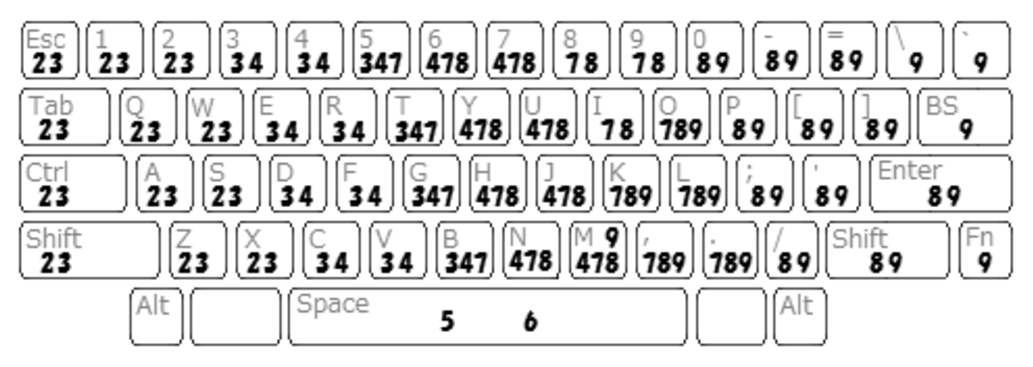
\includegraphics[width=14cm,clip]{res_o_ck/fig2_unsikyoso.eps}
 \end{center}
 \caption{運指表 (勃起教教祖さん)}
 \label{fig2_unsikyoso}
\end{figure*}

\question{それでは、運指表の中身についてツッコミを入れて(?)行きたいと思います。図\ref{fig2_unsikyoso}が教祖さんの運指表になります。
まず気付いたのは、\finger{3}、\finger{4}、\finger{7}、\finger{8}のカバーしている範囲が非常に多いという点で
なんとなく私の運指と近いものを感じました。教祖さんも私と同じように、
同じキーを違う指で打鍵するということが頻繁にあるのでしょうか?
(例えば、本記事にもある tetyou(\finger{433487}) における\key{T}キーのように)}


\answer{教祖}{大いにあります。
同じワードの例でいうと、tetyouは\finger{434787}です。
左手よりも右手の方がよく動くため、どうしても右手に偏ってしまいますが、
隣接するキーは頻繁に同じ指で担当します。
また、移動する距離も比較的広いです。}



\question{左\key{Shift}キーは\finger{2}&\finger{3}とありますが、小指は一切使わないのですか?
左右の\key{Shift}キーを使い分けしているのでしょうか。}


\answer{教祖}{小指で\key{Shift}キーが押せません。\key{Shift}キー使い分けはしています。
主に左端のキーを使う際は、一部は左\key{Shift}キーを。
それ以外のほとんどは右\key{Shift}キーを。逆も同様です。}



\question{\key{Space}キーが\finger{5}&\finger{6}とありますが、これも使い分けしているのでしょうか。}


\answer{教祖}{はい。主に負担の軽い方の手の親指を使っています。
ただ、体感は左親指の方が多いです。理由としては、右手の方がメインのキーで手一杯なことが多いからです。}



\question{ご自身の運指で利点、欠点と考えられる点があれば教えて下さい。
また一風変わった加速ワードや、もしくは意外な苦手ワードもおありでしたら是非!}


\answer{教祖}{自分が使う上では、一番使いやすい運指が今のものなので、欠点らしいものはありません。
一般的な見方でいう欠点なら、先ほどあげた通り沢山あります。

加速ワードについてですが、「ありがとうございました。」等の会話ワードは得意です。
中でも、\key{A}が頻繁に入ってくるワードに関しては、左薬指を\key{A}で固定している関係上、
非常に加速できます。

苦手なワードについてですが、記号全般です。トラウマ的なものを、今もひきずっています。
PC版TODが出た当時、カエルという記号類を打つ種目があったのですが、
あれが絶望的なまでに苦手でした。}



\question{小指ってどうですか?(運指的な意味で)}


\answer{教祖}{小指なんてなかった}



\question{使用しているキーボードについて、こだわりがあれば教えて下さい。
ちなみに、私はもうパンタグラフしか愛せません!}


\answer{教祖}{キー配置を覚えた当時のキーボードが、PC9821付属の物凄く大きいキーボードで、
今もキーボードの大きさにはこだわっています。
また、キーの間隔にも余裕があり、キー自体の厚みがあるものが好みです。
同じ理由で、GATEWAYのG9900には、本当に長い間お世話になりました。
今は、cherryのメカニカルスイッチを使ったキーボードを使っています。
あのクリック感が大好きですね。
また、テンキーレスモデルは個人的に好きではありません。
エルゴノミクスキーボードは、運指の関係上まったく使い物になりません。
加えて、ノートパソコン付属のキーボードだと、窮屈すぎて速度が2割ぐらいになります。
最後に、\key{Space}キーが短いキーボードは許せませんね。
店頭展示品を試打した際に、\key{Space}キーに親指が届かないものがあったりして困りました。


余談ですが、ゲーミングキーボードと銘打って販売されている商品が多数あるのですが、
それらが悉く不出来な事に最近イライラしています。}



\question{最近はタイピングをあまりなさっていない様子ですが、
なにか理由がおありなのでしょうか。(事故による怪我の影響という噂も…?)
タイピング復帰を望む声もあるかと思いますが、復帰の予定はありますか?}


\answer{教祖}{単純に情熱が冷めてしまったことが原因ですね。
事故に関しては、もう傷も癒えています。

昔のように、記録更新に熱くなれなくなったのが致命傷だと思います。
情熱が冷めてしまっては、モチベーションも何もないので。
当時だと、記録が破られたら抜き返そうという意欲が沸いたのですが、
残念ながら今はもうありません。}



\question{本日は、我流運指のトップタイパーによる貴重な意見をどうもありがとうございました!
最後に、上達を目指しているタイパーの方々に向けて一言お願いします。}


\answer{教祖}{原則や普通というものを重視することもいいけれど、ある程度上達したところで、
独自色を出していくのも重要なのではないかと思います。
打鍵について、自分だけのこだわりです。
自分の打ち方で誇れるものは何か。何が得意で、これからどう進化させたいか。


他の人と比較をしたり、違う視点からアプローチをする等で、
自分だけのタイピング観のようなものができると思います。
これなら負けない。そう胸を張れるものが自分の中にできればいいなと思います。
あとは、自分を信じてひたすらキーボードに触れるのみです。
結局のところ、上達しようと思ったら、モノに触れる時間を増やさないとダメですからね。}

\newpage

あらためて教祖さん、お忙しいところインタビューに答えてくださり、本当にどうもありがとうございました!
「wazawaza \finger{43734373}」には大変驚かされました(笑) 以下、今回のインタビューを通して
私が思った感想を少しだけ書いてみたいと思います。


人差し指・中指を多用しているということだけでなく、自然にタッチタイプを覚え無意識的に
運指が構築されていったということ、また記号に苦手意識を持っていることなど、
私と共通点が多いように感じました。
しかし、\key{Space}キーを両方の親指で使い分けしているという点については
面白いなと思いました。私は今まで「左右どちらでも大して変わらないだろう」くらいにしか
思っていませんでしたが、確かに\key{Space}キーに関しても、左右の手で打ち分けができるようになれば、
タイプウェルのようなゲームだけでなく、実用においてもさらに快適に打つことができるかもしれませんね。


「キーボードが固い」というのも、これまた人差し指・中指を多用するような我流運指が生まれる
理由のひとつになり得そうですね。これには私は気が付きませんでした。
確かに、公共のパソコンに付属しているようなメンブレンのキーボードって、
たまに尋常じゃないくらいキータッチが固いやつありますね…(笑)


我流運指はもちろんメリットだけでなく、それに伴うデメリットもあるわけですし、
“人に薦める”という類のものではないと思います。
しかし、何事も“型にとらわれない”考え方というのもまた大事で、
「このほうが打ちやすそうだな」と思った最適化は、まずは実際に手を動かして
試してみれば、頭の体操になって新しい発見が得られるかもしれません。


本記事を通して、読者の方々に“自分だけのタイピング観”について
あらためて考えるきっかけとなれば、幸いです。



\section{おわりに}

タイピングは、私の人生を変えてくれたもののひとつだと、断言できます。
パソコンを使う様々な場面で役に立つというだけでなく、
タイピングを通して自分の可能性を発見できたり、なにより同じ趣味を通して
日本中のタイパーと交流する機会を与えてくれた、素晴らしい趣味だと感じています。


今回、tomoemonさんからご依頼を頂いて、タイピング本に記事を執筆させて頂くことになったのも
タイピングという趣味を通しての縁があってこそと思います。一連の企画の主催であるtomoemonさん、
本当にどうもありがとうございました。

また、インタビューを快く引き受けてくださった勃起教教祖さん、並びに、我流運指の考察について
雑談を交えながらあれこれと議論に付き合っていただいた、クリームさん、paraphrohnさん、
のんさん、eighさん、Saifosさん、みこやんさん、ありがとうございました。
この場を借りて御礼申し上げます。


本記事が、読者の皆さんにとって新たな知見となり、またタイピングへのモチベーション向上の
きっかけとなれば、執筆者として冥利に尽きます。

タイピング界のさらなる発展を祈りつつ、以上を結言とさせて頂きます。
ありがとうございました。

2011年10月 o-ck
